\section{Introduction}

Many real world Bayesian inference problems such as preference learning, predicting traders’ behavior in a financial market, competitive skill learning, etc. naturally have piecewise likelihood and/or prior models. To date tools for carrying out Bayesian reasoning in such models are either approximate (namely, approximate message passing with Gaussian priors/posteriors) or unscalable. The latter group consists of sampling-based methods limited to Metropolis-Hastings and rejection sampling. They are considered unscalable since in many models their convergence rate is slow (in time). 
This is particularly true if they are not tunned well, in the sense that 
a ``proper" \emph{envelope distribution} (or \emph{proposal distribution}) 
which is required for rejection sampling (resp. Metropolis-Hasting samplings) is not chosen.
In practice, such a tunning can be difficult and problem-dependent. 
Gibbs sampling, on the other hand, does not require tunning, and in this sense, is robust.
Nonetheless, in piecewise models and in particular when likelihood models are piecewise,
the time/space computation costs of Gibbs sampling can grow exponential in the amount of observed data.    This is prohibitively expensive 
and to our knowledge, so far, Gibbs sampling has not been used in the aforementioned models. 

Our work fills this gap by providing a Bayesian inference method which is both scalable and asymptotically unbiased that can be used in a large family of piecewise Bayesian models. 
In particular, the presented method reveals its superiority over the existing tools where the number of partitions in a piecewise distribution is huge.    

To motivate the need for piecewise models, consider the following running example:
%%%%%%%%%%%%%%%%%%%%%%%%%
\begin{figure}%[t!]
\centering
\begin{subfigure}{.2\textwidth}
  \centering
  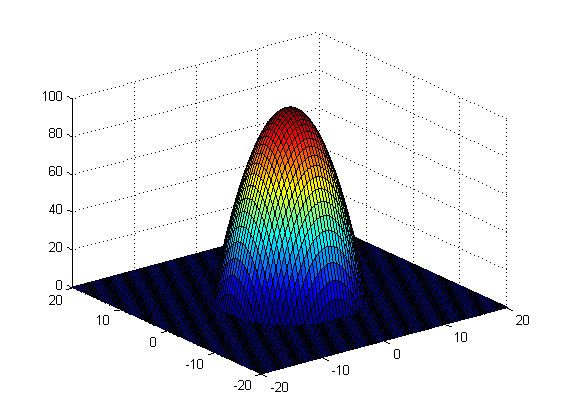
\includegraphics[width=.99\textwidth]{pic/bpplPriorII.png}
  \label{fig:prior2d}
\end{subfigure}%
\begin{subfigure}{.58\textwidth}
\centering
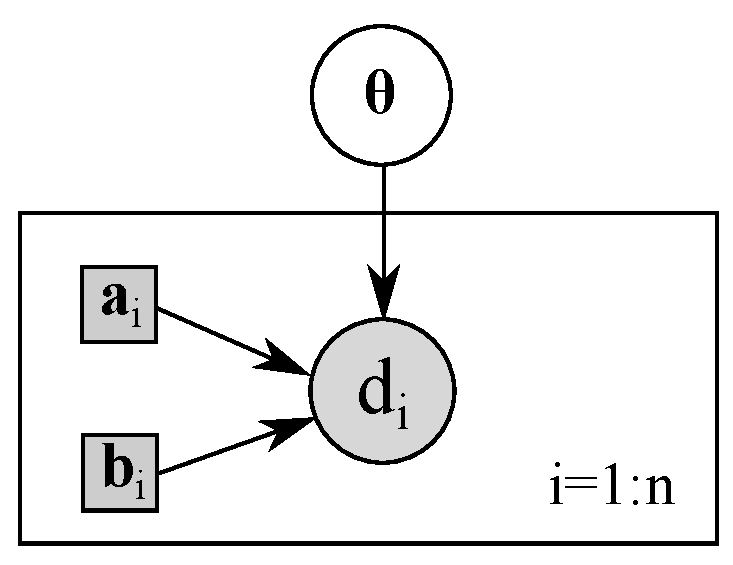
\includegraphics[width=.24\textwidth]{pic/pref2w.pdf}
\caption{\footnotesize Graphical model for BPPL problem in Example \ref{example:pref}. }
\end{subfigure}
\begin{subfigure}{.2\textwidth}
  \centering
  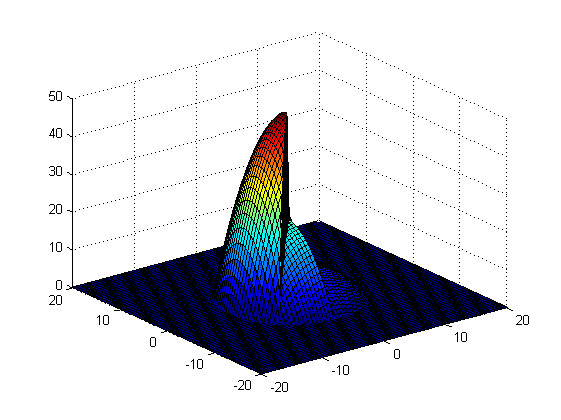
\includegraphics[width=.99\textwidth]{pic/bpplPosteriorII.png}
  \label{fig:prior2d}
\end{subfigure}%
\label{fig:pref}
\end{figure}
%%%%%%%%%%%%%%%%%%%%%%%%%
\begin{figure}%[t!]
\centering
\begin{subfigure}{.2\textwidth}
  \centering
  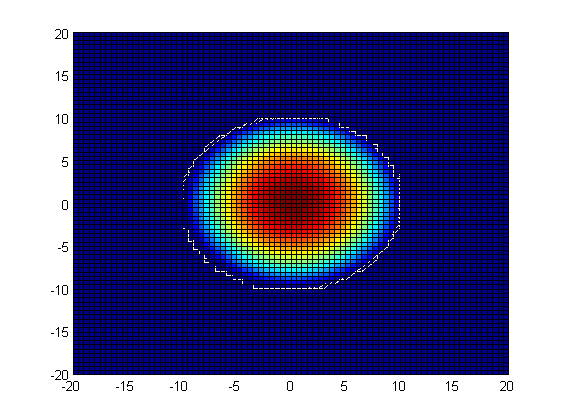
\includegraphics[width=.99\textwidth]{pic/bpplPriorART.png}
  \label{fig:prior2d}
\end{subfigure}%
\begin{subfigure}{.58\textwidth}
\centering
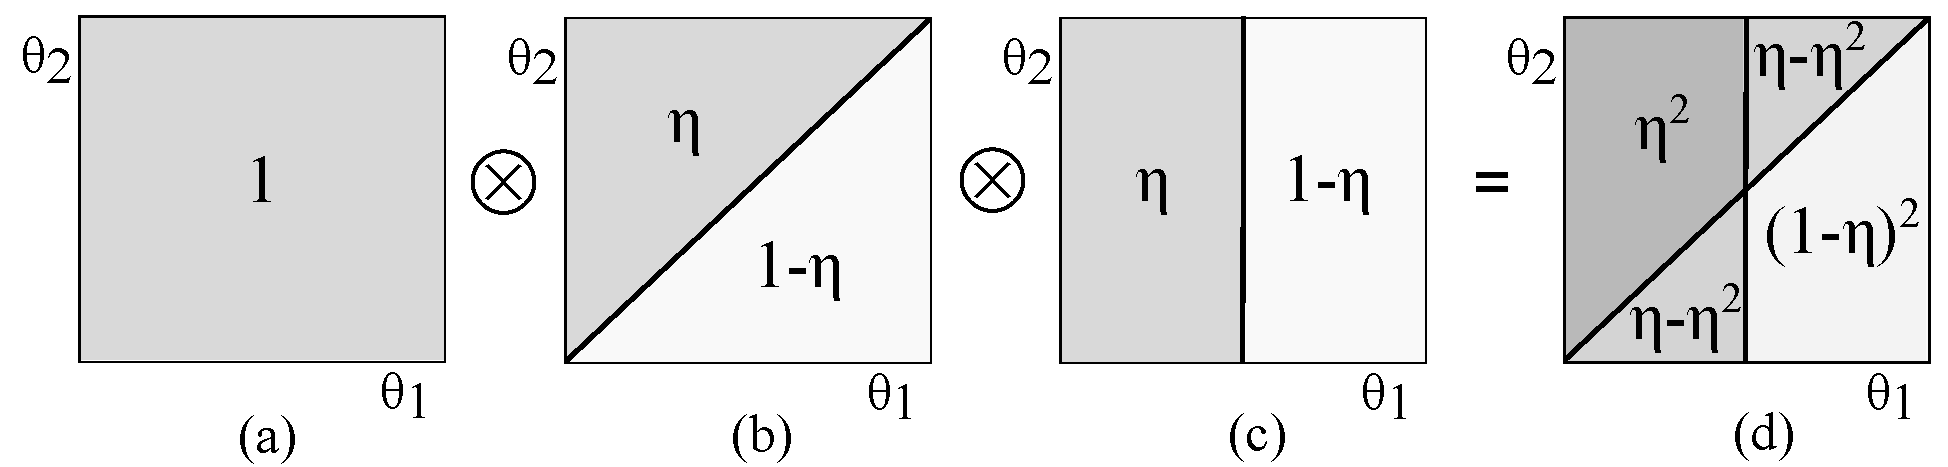
\includegraphics[width=.99\textwidth]{pic/running1.pdf}
\end{subfigure}
\begin{subfigure}{.2\textwidth}
  \centering
  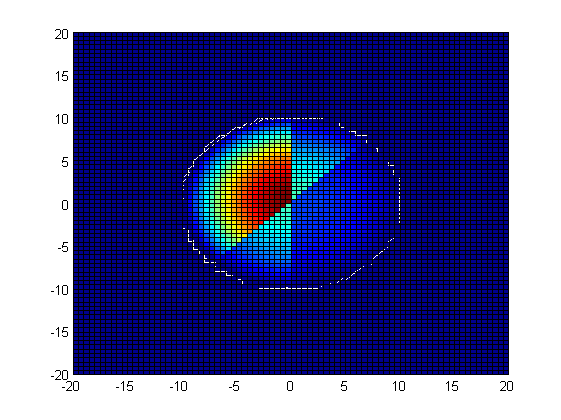
\includegraphics[width=.99\textwidth]{pic/bpplPosteriorIII.png}
  \label{fig:prior2d}
\end{subfigure}%
\caption{\footnotesize A 2D instance of Example \ref{example:pref}. 
(a) A (non-normalized) prior uniform in a hyperrectangle with center (0,0).
(b) Likelihood model $pr(\bvec{a}_1 \succ \bvec{b}_1 | \, \boldsymbol\theta)$ and
(c) $pr(\bvec{a}_2 \succ \bvec{b}_2 | \, \boldsymbol\theta)$ 
(as in equation~\ref{e:pref1likelihood}) where
$\bvec{a}_1 = (5, 3)$, $\bvec{b}_1 = (6, 2)$, $\bvec{a}_2 = \bvec{a}_1$ and $\bvec{b}_2 = (6, 3)$.
(d) A piecewise function proportional to the posterior distribution.}
\label{fig:pref-up-down}
\end{figure}
%%%%%%%%%%%%%%%%%%%%%%%%%
\fexample{example:pref}{Bayesian pairwise preference learning (BPPL)}{
Suppose each \emph{item} $\bvec{a}$ is an $N$-dimensional real-valued \emph{attribute choice vector} 
$(\alpha_1, \ldots, \alpha_N)$.
The goal is to learn an \emph{attribute weight vector} 
$\boldsymbol\theta = (\theta_1, \ldots, \theta_N) \in \mathbb{R}^N$ 
that describes the utility of each attribute choice from user responses to preference queries.
As commonly done in \emph{multi-attribute utility theory} \cite{Keeney:93},
the overall item utility $u(\bvec{a}|\, \boldsymbol\theta)$ decomposes additively over the attribute choices of $\bvec{a}$:
%
$$
u(\bvec{a} | \, \boldsymbol\theta) = \sum_{j=1}^N \theta_j \cdot \alpha_j
$$
%
User responses are in the form of $n$ queries (i.e.\ observed data points) $d_1$ to $d_n$ where $d_i$ is a pairwise comparison of some items $\bvec{a}_i$ and $\bvec{b}_i$ with the following possible 
responses: 
\begin{itemize}
\item $\bvec{a}_i \succ \bvec{b}_i$:  In the $i$-th query, the user prefers item $\bvec{a}_i$ over $\bvec{b}_i$.
\item $\bvec{a}_i \preceq \bvec{b}_i$:  In the $i$-th query, the user does not prefers item $\bvec{a}_i$ over $\bvec{b}_i$.
\end{itemize}
It is assumed that with an \emph{elicitation noise} $0 \leq \eta < 0.5$, the item with a greater overall utility is preferred:
\begin{equation}
\label{e:pref1likelihood}
pr(\bvec{a}_i \succ \bvec{b}_i \,|\, \boldsymbol\theta) =
{\footnotesize
\begin{cases}
u(\bvec{a}_i|\boldsymbol\theta) < u(\bvec{b}_i|\boldsymbol\theta) : \eta\\
u(\bvec{a}_i|\boldsymbol\theta) = u(\bvec{b}_i|\boldsymbol\theta) : 0.5\\
u(\bvec{a}_i|\boldsymbol\theta) > u(\bvec{b}_i|\boldsymbol\theta) : 1-\eta
\end{cases}
}%end footnote size
\quad
pr(\bvec{a}_i \preceq \bvec{b}_i \,|\, \boldsymbol\theta) = 
1 - pr(\bvec{a}_i \succ \bvec{b}_i \,|\, \boldsymbol\theta)
\end{equation}
As the graphical model in Figure~(\ref{fig:pref}) illustrates:
$
pr(\boldsymbol\theta | \, d_1, \ldots, d_n) 
\propto pr(\boldsymbol\theta) \cdot \prod_{i=1}^{n} pr(d_i | \, \boldsymbol\theta)
$.
} %end example 1
\vspace{2mm}
%%%%%%%%%%%%%%%%%%%%%%%%%%%%%%%%%%%%%%%%
Since in the above example, likelihood  models are piecewise, 
as Figure~(\ref{fig:pref-up-down}) illustrates, the posterior distribution is also piecewise.
However, the number of partitions in the posterior grow exponential as the number of likelihoods grow.
In the following it will be shown that such a complexity not only prohibits exact inference to be carried out on piecewise modes with large number of observed points, but also the speed and convergence rate of asymptotically unbiased methods can be negatively affected.
Based on our experiments, in particular, the speed of \emph{Gibbs sampling} 
(and to a lesser extend, \emph{rejection sampling}) rapidly decreased as the number of observed data points increase.
In this paper, we will present a variation of Gibbs sampling with an exponential-to-linear reductions in the amount of computations performed in each sampling step. 
The core insight is that by treating each piecewise factor as a mixture distribution single-piece distributions and carrying out Gibbs sampling on such a model. 
This is equivalent with limiting the number of ``active" partitions in each step of sampling rather than dealing with the total space.
After introducing piecewise functions and the exact/asymptotically unbiased inference methods that can be used on piecewise modes, in Section~\ref{sec:inference_piecewise_models}, the new algorithm (referred to as \emph{Augmented Gibbs} sampling throughout) is presented.
The performance of this algorithm against other sampling methods is tested in Section~\ref{???} 
on BPPL and another piecewise models. 
It is seen that on these models, \emph{augmented Gibbs} is also scalable in the dimension of the parameter space while for instance \emph{Metropolis-Hastings} sampling method is not.
Finally Section~\ref{???} concludes.
